\documentclass{ceri}
\usepackage{xcolor}

%%%%%%%%%%%%%%%%%%%%%%%%%%%%%%%%%%%%%%%%%%%%%%%%%%%
%% Informations générales
%%%%%%%%%%%%%%%%%%%%%%%%%%%%%%%%%%%%%%%%%%%%%%%%%%%
\title{Projet d’optimisation}    
\author{
	MATHIEU Thomas et REZAIGUI Nizar
}
\classname{Algorithme et optimisation} 
\formation{Licence informatique}
\parcours{Licence 2}

\begin{document}

% création de la page de titre

\maketitle

\parindent=0cm
% création de la table des matières
\MyToc

% Justification moins stricte : des mots ne dépasseront pas des paragraphes
\sloppy          


%%%%%%%%%%%%%%%%%%%%%%%%%%%%%%%%%%%%%%%%%%%%%%%%%%%
%% Introduction
%%%%%%%%%%%%%%%%%%%%%%%%%%%%%%%%%%%%%%%%%%%%%%%%%%%
\section{Introduction}
Le groupe qui va traité de ce problème se compose de deux personnes :
-	Rezaigui Nizar,
-	Mathieu Thomas.\\

Tous deux, sont étudiants à la fac d'Avignon sur le campus d'Agroparc. Ils sont étudiants en informatique et vont traités à travers ce document d'un problème d'algorithmique et d'optimisation.\\

Le sujet que nous avons eu, porte sur Volkswagen of America et sur les problèmes qu'ils ont rencontrés\\
Nous allons maintenant vous expliquer le problème de cet entreprise.
\clearpage

\section{Problème}

L'article «Analyse de la chaîne d'approvisionnement chez Volkswagen of America» donne un aperçu du système de distribution existant de Volkswagen of America et précise également les opportunités de changement avec des économies significatives.\\


En 1995, Volkswagen of America a chargé une équipe de projet d'évaluer le processus de distribution de véhicules existant et de développer un nouveau modèle de distribution amélioré.\\


Les objectifs de l'entreprise étaient d'améliorer la réactivité et de réduire les coûts d'un client à l'autre dans le monde entier.\\
Volkswagen of America, une filiale de Volkswagen AG (Allemagne), importe et distribue des véhicules Volkswagen et Audi aux États-Unis.\\
Les véhicules assemblés au Mexique ou en Allemagne sont distribués à un réseau de concessionnaires Volkswagen à travers les États-Unis.\\


Les auteurs soulignent que le système de distribution existant a servi l'entreprise pendant de nombreuses années et n'a presque jamais été examiné.\\
L'argument principal est que le système actuel n'a pas été conçu pour maximiser le profit pour l'ensemble du système, mais seulement pour réaliser des flux de trésorerie pour la fabrication d'origine.\\
En effet, il date des années ou Ford avait commencé à définir ce sujet, à l'époque tout le monde l'avait trouvé super, mais jamais personne ne l'avait examiné de plus prêt.\\


C'est-à-dire que l'intérêt n'était que le bénéfice de la fabrication plutôt que l'avantage pour Volkswagen et les concessionnaires des États-Unis réunis.\\
Le système de distribution existant aux États-Unis "a une forme dominante unique, dans lequel l'équipement d'origine fabrique (OEM) inventaire et vendre de nouveaux véhicules aux vendeurs franchisés." \\
Ainsi, le concessionnaire était un client principal pour une Volkswagen, et le concessionnaire étaitun fournisseur à l'utilisateur final.Par conséquent, les concessionnaires et les équipementiers n'étaient que vaguement attachés au système, ce qui créait de nombreux désavantages pour les deux parties.\\


Les concessionnaires étaient encouragés à faire le plus d'inventaire possible, même s'ils se rendaient compte que cela menaçait leurs entreprises.De plus, ils dépendaient des OEM parce qu'ils pouvaient restreindre l'approvisionnement ou désigner des concessionnaires concurrents.\\
Cette logique de distribution spécifique a été développée en supposant que les véhicules étaient configurés comme un modèle de ligne de produits standardisé en une couleur.(Ford avait initiiez ce mode de fonctionnement)\\


Même après l'introduction d'un avantage concurrentiel dans le réseau, la structure du système de distribution était restée la même.\\
Le résultat de cette structure était que les concessionnaires n'étaient pas en mesure d'offrir au client un produit réellement requis en raison de l'inventaire limité, même si les fabricants de la dernière décennie ont commencé à offrir des milliers de modèles.\\


Le sujet de cet article est une étude sur une nouvelle configuration qui pourrait faire face à ces limitations et réaliser des bénéfices pour Volkswagen et les concessionnaires ensemble.\\

Les objectifs comprenaient :\\
- la maximisation du pourcentage de clients recevant leur premier choix de véhicules,\\
- la livraison en moins de 48h pour limiter les inventaires,\\
- livrer a partir des stocks de Volkswagen ou d'autres afin de minimiser les coûts.\\


En réduisant les stocks, l'objectif était de réduire les coûts totaux du système pour les concessionnaires et Volkswagen, y compris les coûts de transport, de financement et de stockage.\\

\clearpage
\bigskip

\section{Méthode de solution}

Une solution possible consistait à regrouper les véhicules dans des dépôts régionaux afin de réduire les stocks des concessionnaires locaux et de garantir la livraison dans les 48 heures.Ainsi, le système augmenterait les ventes de premier choix, serait opportun et réduirait les coûts d'inventaire.\\


Cependant, Volkswagen n'avait aucun moyen efficace de tester ce système pour la faisabilité. La complexité et la portée du système ont rendu l'analyse statique de valeur limitée.\\


Ainsi, l'équipe de l'étude a identifié la simulation comme un moyen potentiellement efficace de tester le modèle et divers scénarios de mise en œuvre :\\
- les véhicules destinés à la vente seraient d'abord expédiés dans cinq ports américains qui agiraient comme des centres de distribution. (puis par des voies ferres),\\
- transport des véhicules par train ou par camion à des concessionnaires à travers les États-Unis.(avoir le plus de centre de distribution proches des métropoles afin de tester la théorie selon laquelle cela augmenterait la demande et minimise les coûts).\\


Tous les facteurs conduiraient à réduire les coûts totaux du système et à accroître la réactivité du client. Le système décrit par les auteurs consiste en des cycles de flux de clients et de circulation de véhicules.\\
Ce cycle définit le niveau de service du client, dans ce cycle, les clients arrivent chez le concessionnaires, demandent un véhicule spécifique, si ce dernier est disponible dans ce magasin cela est un avantage concurrentiel énorme, de plus si par hasard il ne l'a pas, il suffit au concessionnaire de le commander et il le reçoit dans les 24h.\\


Pour mener à bien ce projet, il fallait mettre en place des centres de traitements et de distribution qui sont les principaux facteur affectant ce cycle :\\
- installation de première catégories (plus petite / moins chère)\\
- installation de deuxième catégories (plus grand / plus chère)\\


Pour la réalisation de ce projet, le groupe d'étude qui a mené ce projet à créer plusieurs scénario sur la localisation et les emplacements des centres de de distribution et de traitement en fonction de leurs situation géographique, la demande des clients au cour de l'année, le retard des transport qu'il pourrait y avoir et plein d'autres éléments afin de pouvoir parer à toute évantualité.\\
Ils ont utilisé un modèle de simulation pour considérer les deux éléments. Le modèle incluait les cycles client et véhicule pour calculer les mesures de performance :\\
- nombre de concessionnaires a été divisé en 52 principales zones de demande,\\
- ils ont défini 50 produits, chacun représentant une famille de véhicules présentant des caractéristiques similaires,\\
- l'équipe a analysé les données de ventes passées pour calculer la variation de la demande au cours d'une année.\\



L'équipe d'étude a identifié 18 emplacements potentiels pour les centres de traitement et de traitement des données aux États-Unis, y compris les cinq ports actuels.\\

Afin de réduire le nombre de scénarios de localisation alternatifs à évaluer, l'équipe a formulé un programme d'entiers mixtes (MIP) qui a généré un nombre raisonnable de scénarios.
La formulation a été personnalisée à partir du problème de charge fixe bien connu. La façon dont MIP fonctionnait était minimisée "une fonction de coût qui approximait le coût de distribution du système réel en ignorant les éléments stochastiques et dynamiques." \\
La sortie du MIP était un scénario de localisation.\\


Donn\'ees :\\


Dij\ \ \ \ Avec \textbf{v} la demande d'un v\'ehicule. Dans le centre \textbf{j}

Mij\ \ \ \ distance entre le distributeur \textbf{i} et le vendeur \textbf{j}

C1sk\ \ \ \ cout du de la livraison de la source \textbf{s} au centre \textbf{k}

C2ki\ \ \ \ cout de la livraison d'un v\'ehicule \textbf{k} au centre de location \textbf{i}

Lj\ \ \ \ chargement d'un facteur pour un magasin \textbf{j}

T1\ \ \ \ prix fixe d'un camion\ \ \ \ \$/truck.

T2\ \ \ \ prix variable d'un camion \$/truck/miles.

Fit\ \ \ \ prix annuel de l'op\'eration et d'installation d'un produit de type \textbf{t} dans un centre de  distribution \ \ \ \ \textbf{i}.

\ \ \ \ (t =1 for type 1 ,,,)

Gk\ \ \ \ prix annuel de l'op\'eration et de l'agent immobilier

\ \ \ \ d'installation d'un produit dans un centre de distribution

Ci\ \ \ \ annuel capacit\'e de transport d'un type 1 vers un center location \textbf{i}

X1skv\ \ \ \ logistique annuel de v\'ehicule \textbf{v }depuis sa source\textbf{s} vers le processus center location 

X2kiv\ \ \ \ logistique annuel de v\'ehicule \textbf{v }depuis processus center \textbf{k} vers distribution center \textbf{i}.

X3ijv\ \ \ \ logistique annuel de v\'ehicule \textbf{v }depuis processus center location \textbf{i} vers le \ \ \ \ \ \ marcher location

\bigskip

\ \ \ \ \ \ {\textbar}\ \ \ \ 1 \ \ si type \textbf{t} est installer dans le centre de distribution / location \textbf{i}.

Yit

\ \ \ \ \ \ {\textbar}\ \ \ \ 0 sinon

\bigskip

\ \ \ \ \ \ {\textbar}\ \ \ \ 1 \ \ si un processus center est installer sur \textbf{k}

Zk\ \ 

\ \ \ \ \ \ {\textbar}\ \ \ \ 1 \ \ 0 sinon

\bigskip
\bigskip
\bigskip
\bigskip
\bigskip
\begin{figure}
\centering
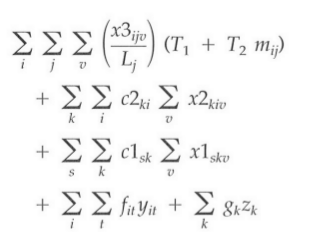
\includegraphics[width=7cm]{t1.png}
\caption{\label{fig:t1}Minimise le coût total combiné, des transport et des installations fixes en Amérique}
\end{figure}

\begin{figure}
\centering
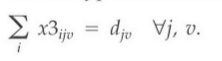
\includegraphics[width=7cm]{t2.png}
\caption{\label{fig:t2}Calcul de la demande de chaque magasin pour chaque type de véhicule}
\end{figure}

\begin{figure}
\centering
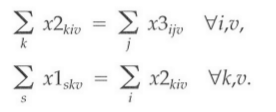
\includegraphics[width=7cm]{t3.png}
\caption{\label{fig:t3}Flux de véhicule du centre de fabrication vers le centre d'action et de distribution}
\end{figure}

\begin{figure}
\centering
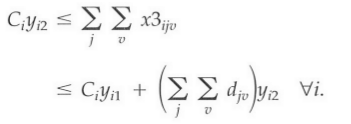
\includegraphics[width=7cm]{t4.png}
\caption{\label{fig:t4}Total de véhicule entre le centre de distribution doit satisfaire le minimun et maximum de capacité que requiert le type de centre installé}
\end{figure}

\begin{figure}
\centering
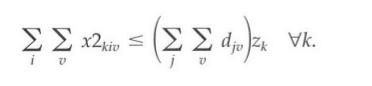
\includegraphics[width=7cm]{t5.png}
\caption{\label{fig:t5}Aucun bateau et autorisé à être dans un centre d'action si aucun centre n'est installé. Vérifie que le quantité de bateau soit supérieur à 0}
\end{figure}

\begin{figure}
\centering
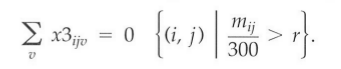
\includegraphics[width=7cm]{t6.png}
\caption{\label{fig:t6}Les centres de distribution doivent être séléctionnées afin que chaque zone du marché peuvent être atteintes en l'espace de r jour}
\end{figure}

\begin{figure}
\centering
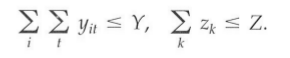
\includegraphics[width=7cm]{t7.png}
\caption{\label{fig:t7}L'endroit choisi doit comprendre soit un centre de distribution / action / les deux}
\end{figure}

\begin{figure}
\centering
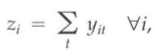
\includegraphics[width=7cm]{t8.png}
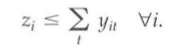
\includegraphics[width=7cm]{t9.png}
\caption{\label{fig:t8}Pour n'importe quel centre de distribution un centre d'action doit être installé}
\end{figure}

Après avoir rentré ces valeurs dans le MIP, plusieurs scénario sortaient ou il localisé les emplacements des centres.\\
L'équipe a tout d'abord conçu le meilleur scénario, puis a généré un certain nombre de scénarios intermédiaires qui définissaient un chemin à suivre du scénario existant au scénario idéal.\\


Dans le premier scénario, ils ont supposé que tous les véhicules devaient passer par des centres de traitement, ce qui était un cas courant, puis à DC. Le nombre maximum de DC a été fixé à six. Le scénario a produit le DC qui a donné le plus grand profit.\\
D'où, ils ont commencé à augmenter le nombre de DC en ne fixant que les cinq centres existants. Ils ont essayé ce scénario jusqu'à ce que le nouveau DC n'était plus rentable.\\
Dans un autre scénario, ils ont répété cette analyse en supposant que les véhicules n'avaient pas besoin de passer par des centres de traitement, mais qu'ils se rendaient directement à un centre de traitement. 

\bigskip
\bigskip

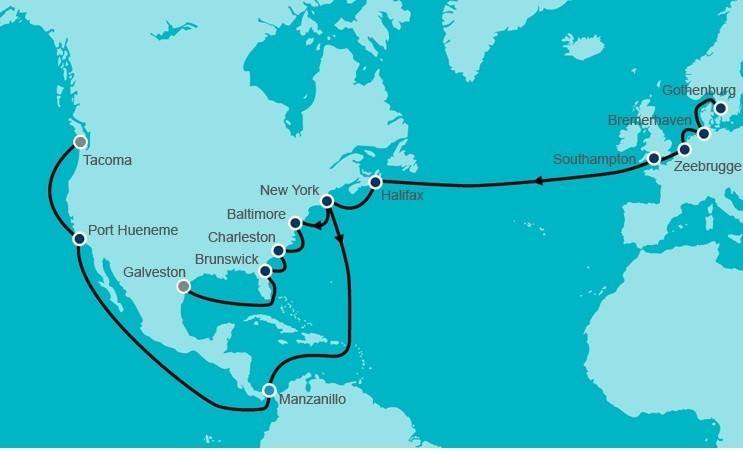
\includegraphics[width=15cm]{monde.jpg}
 
\clearpage
\bigskip

\section{Implémentation}

Pour l’implémentation du sujet , nous avons suivi les indications aux quels en sont venus les spécialistes. Ainsi que les contrainte.\\


	Le sujet est une minimisation des coûts combiner du transport et des  disposition envisageable d’installation fixe, tel que les centre de distribution.\\
Nous avons donc utilisé Julia et Cplex comme solveur. Le package JuMP nous a parmi de mettre des condition tels que pour la contrainte 6.\\


	Le sujet demander a ce que soit appliqué des sommes de matrices de tableaux afin de satisfaire toutes les données mis a dispositions des spécialistes. Pour ce faire ils ce sont aider de calculateur afin de simuler et généré des données puis appliqué les données réelles afin de satisfaire Volkwagen of America.\\
	La simulation semble donné de bon résultat a 6 centres de distributions avec un coûts minimum pour un meilleur transit et expédition vers des concessionnaire regroupé en paquet de 52 concessionnaire a travers le pays.\\
    

	La simulation par intégration du précédent fichiers puis en changeant la variable biaisé, a actuellement révéler plusieurs scénarios différents avec des résultat semblables.\\
	Cette simulation a permis aussi de révéler la position heuristique du sujet. En effet, augmentant de 1 le nombres de centres de distributions jusqu’à n, le nouveaux points optimales était le même que le précédents, sans dire que cella est garantit.\\
	La complexité du sujets, ainsi que les faibles données ne nous ont pas permis de créés de tels instances. Les variables comprises n’ont pas pus être inventer a une tel échelles ainsi que la simulation. \\
	En effet le sujet requière une simulation de changement de variable et non l’essai sur un problème. Ils soulève un problème de données heuristique ainsi et d’application concrète du sujets dans ses proportions et ce en quoi il découle.\\
    
    
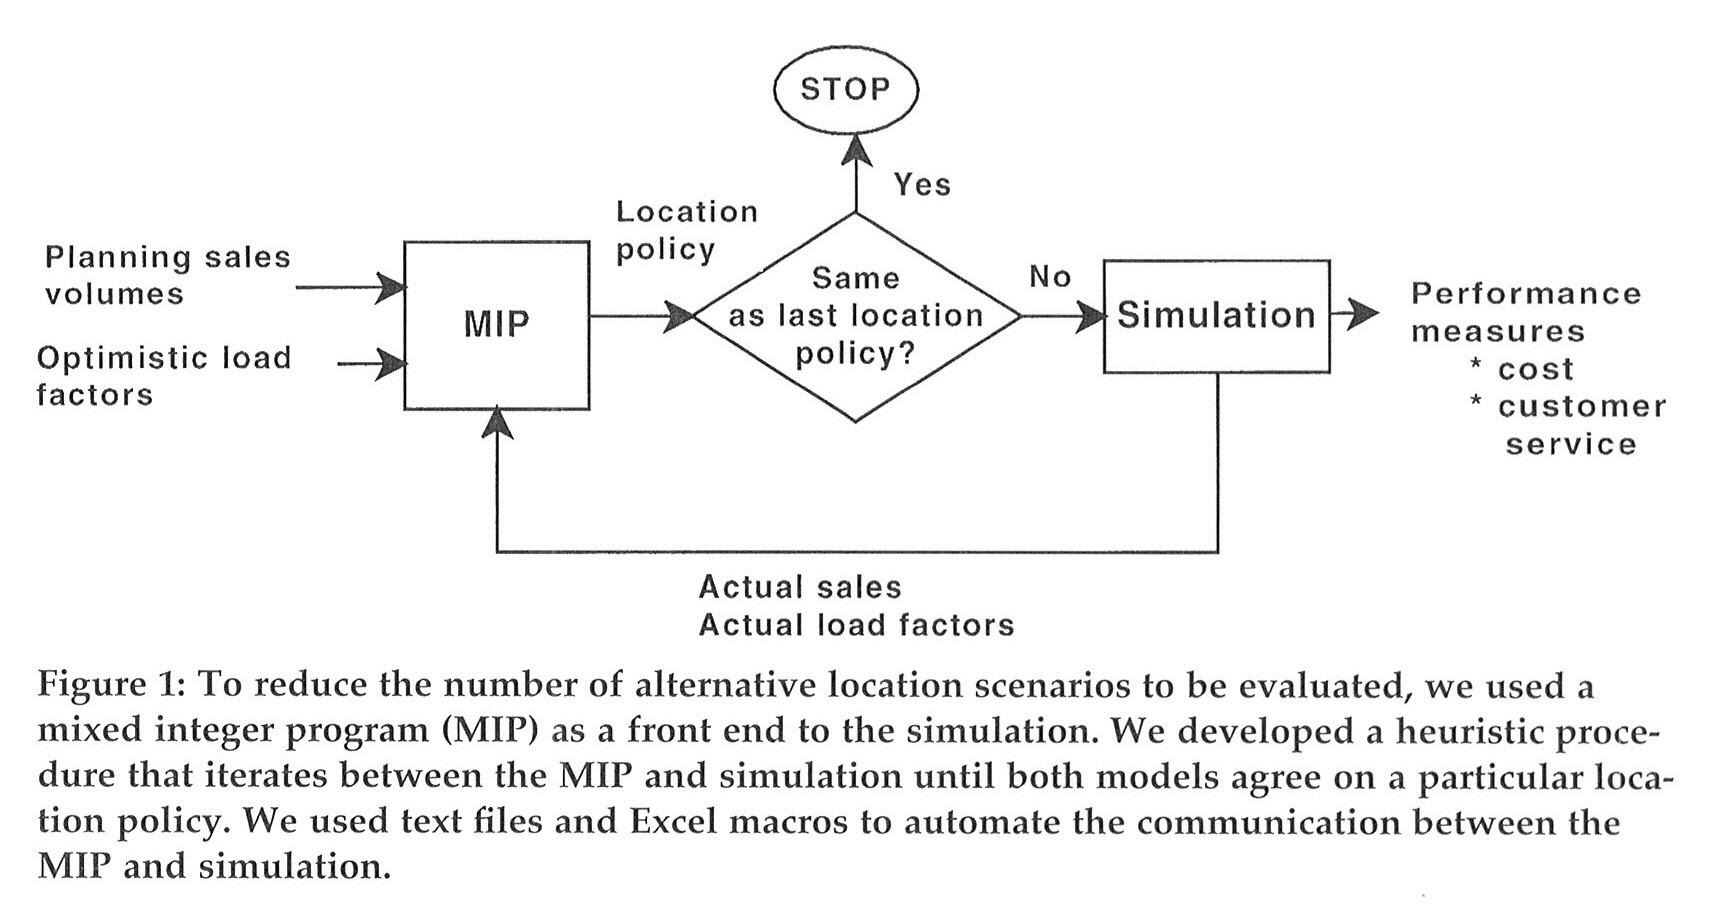
\includegraphics[width=15cm]{donnee.jpg}

\clearpage
\bigskip

\section{Conclusion}

Les principales conclusions des analyses quantitatives basées sur les résultats d'optimisation et de simulation ont montré que certaines modifications apportées à la structure de distribution pourraient amener plus de clients à recevoir des véhicules de premier choix et à réduire simultanément le coût total du système.\\

La conclusion a indiqué que les concessionnaires du sud-est ont réalisé moins d'avantages parce qu'ils se trouvaient à proximité des points d'entrée existants, tandis que les concessionnaires des marchés du Midwest bénéficiaient d'un meilleur service et d'une réduction des coûts.\\
En effet le train étant moins moins chère, le coût optimum a pu monter pour chaque centre de distribution a travers le pays. La nouvelle stratégie n'a pas été acceptée universellement.\\


Par exemple, les concessionnaires du sud-est ont vu la réduction des stocks comme une perte potentielle d'avantage concurrentiel. En 1998, après l'introduction d'un certain nombre de nouveaux modèles sur le marché américain, les DC pilotes n'ont pas été en mesure de maintenir le niveau de stock requis, en raison de la très forte demande.\\


Ainsi, en 1999, le programme pilote a été retiré. Les outils d'optimisation présentaient des opportunités potentielles pour améliorer la chaîne d'approvisionnement en se concentrant sur l'optimisation au niveau du système plutôt que sur le local. \\
Plus important encore, Volkswagen s'est rendu compte que la chaîne d'approvisionnement devait être considérée à partir du système. \\


Le système existant axé sur les flux de trésorerie ne peut que minimiser la rentabilité totale du système et le service à la clientèle. 
\end{document}
